\documentclass[12pt,t]{beamer}
\usepackage{graphicx}
\usepackage{amsmath,amssymb}
\setbeameroption{hide notes}
\setbeamertemplate{note page}[plain]

% get rid of junk
\usetheme{default}
\beamertemplatenavigationsymbolsempty
\hypersetup{pdfpagemode=UseNone} % don't show bookmarks on initial view

% font
%\usepackage{fontspec}
%\setsansfont{TeX Gyre Heros}
%\setbeamerfont{note page}{family*=pplx,size=\footnotesize} % Palatino for notes
% "TeX Gyre Heros can be used as a replacement for Helvetica"
% In Unix, unzip the following into ~/.fonts
% In Mac, unzip it, double-click the .otf files, and install using "FontBook"
%   http://www.gust.org.pl/projects/e-foundry/tex-gyre/heros/qhv2.004otf.zip

% named colors
\definecolor{offwhite}{RGB}{249,242,215}
\definecolor{foreground}{RGB}{255,255,255}
\definecolor{background}{RGB}{24,24,24}
\definecolor{title}{RGB}{107,174,214}
\definecolor{gray}{RGB}{155,155,155}
\definecolor{subtitle}{RGB}{102,255,204}
\definecolor{hilight}{RGB}{102,255,204}
\definecolor{vhilight}{RGB}{255,111,207}
\definecolor{lolight}{RGB}{155,155,155}
%\definecolor{green}{RGB}{125,250,125}
\definecolor{pink}{HTML}{FC0964}
\definecolor{orange}{HTML}{FD971F}
\definecolor{blue}{HTML}{66D9EF}
\definecolor{green}{HTML}{7FB347}


% use those colors
\setbeamercolor{titlelike}{fg=title}
\setbeamercolor{subtitle}{fg=subtitle}
\setbeamercolor{institute}{fg=gray}
\setbeamercolor{normal text}{fg=foreground,bg=background}
\setbeamercolor{item}{fg=foreground} % color of bullets
\setbeamercolor{subitem}{fg=gray}
\setbeamercolor{itemize/enumerate subbody}{fg=gray}
\setbeamertemplate{itemize subitem}{{\textendash}}
\setbeamerfont{itemize/enumerate subbody}{size=\footnotesize}
\setbeamerfont{itemize/enumerate subitem}{size=\footnotesize}

% page number
\setbeamertemplate{footline}{%
    \raisebox{5pt}{\makebox[\paperwidth]{\hfill\makebox[20pt]{\color{gray}
          \scriptsize\insertframenumber}}}\hspace*{5pt}}

% add a bit of space at the top of the notes page
\addtobeamertemplate{note page}{\setlength{\parskip}{12pt}}

% a few macros
\newcommand{\bi}{\begin{itemize}}
\newcommand{\ei}{\end{itemize}}
\newcommand{\ig}{\includegraphics}
\newcommand{\subt}[1]{{\footnotesize \color{subtitle} {#1}}}

% title info
\title{Introduction to Radial Basis Functions}
\subtitle{}
\author{\href{https://github.com/jessebett/}{Jesse Bettencourt}}
\institute{McMaster University}
\date{\href{jessebett@gmail.com}{\tt \scriptsize jessebett@gmail.com}
\\[-4pt]
\href{http://github.com/jessebett}{\tt \scriptsize github.com/jessebett}
}

\graphicspath{{./Images/}}


\begin{document}

% title slide
\setbeamertemplate{footline}{} % no page number here
\begin{frame}
  \titlepage
  \note{}
\end{frame}

\begin{frame}{Motivation}
Given a set of measurments \textcolor{pink}{$\{f_i\}_{i=1}^N$}
taken at corresponding data sites \textcolor{orange}{$\{x_i\}_{i=1}^N$}
we want to find an interpolation function \textcolor{blue}{$s(x)$}
that infroms us on our system at locations different from our data sites.\\
\bigskip 

\begin{figure}
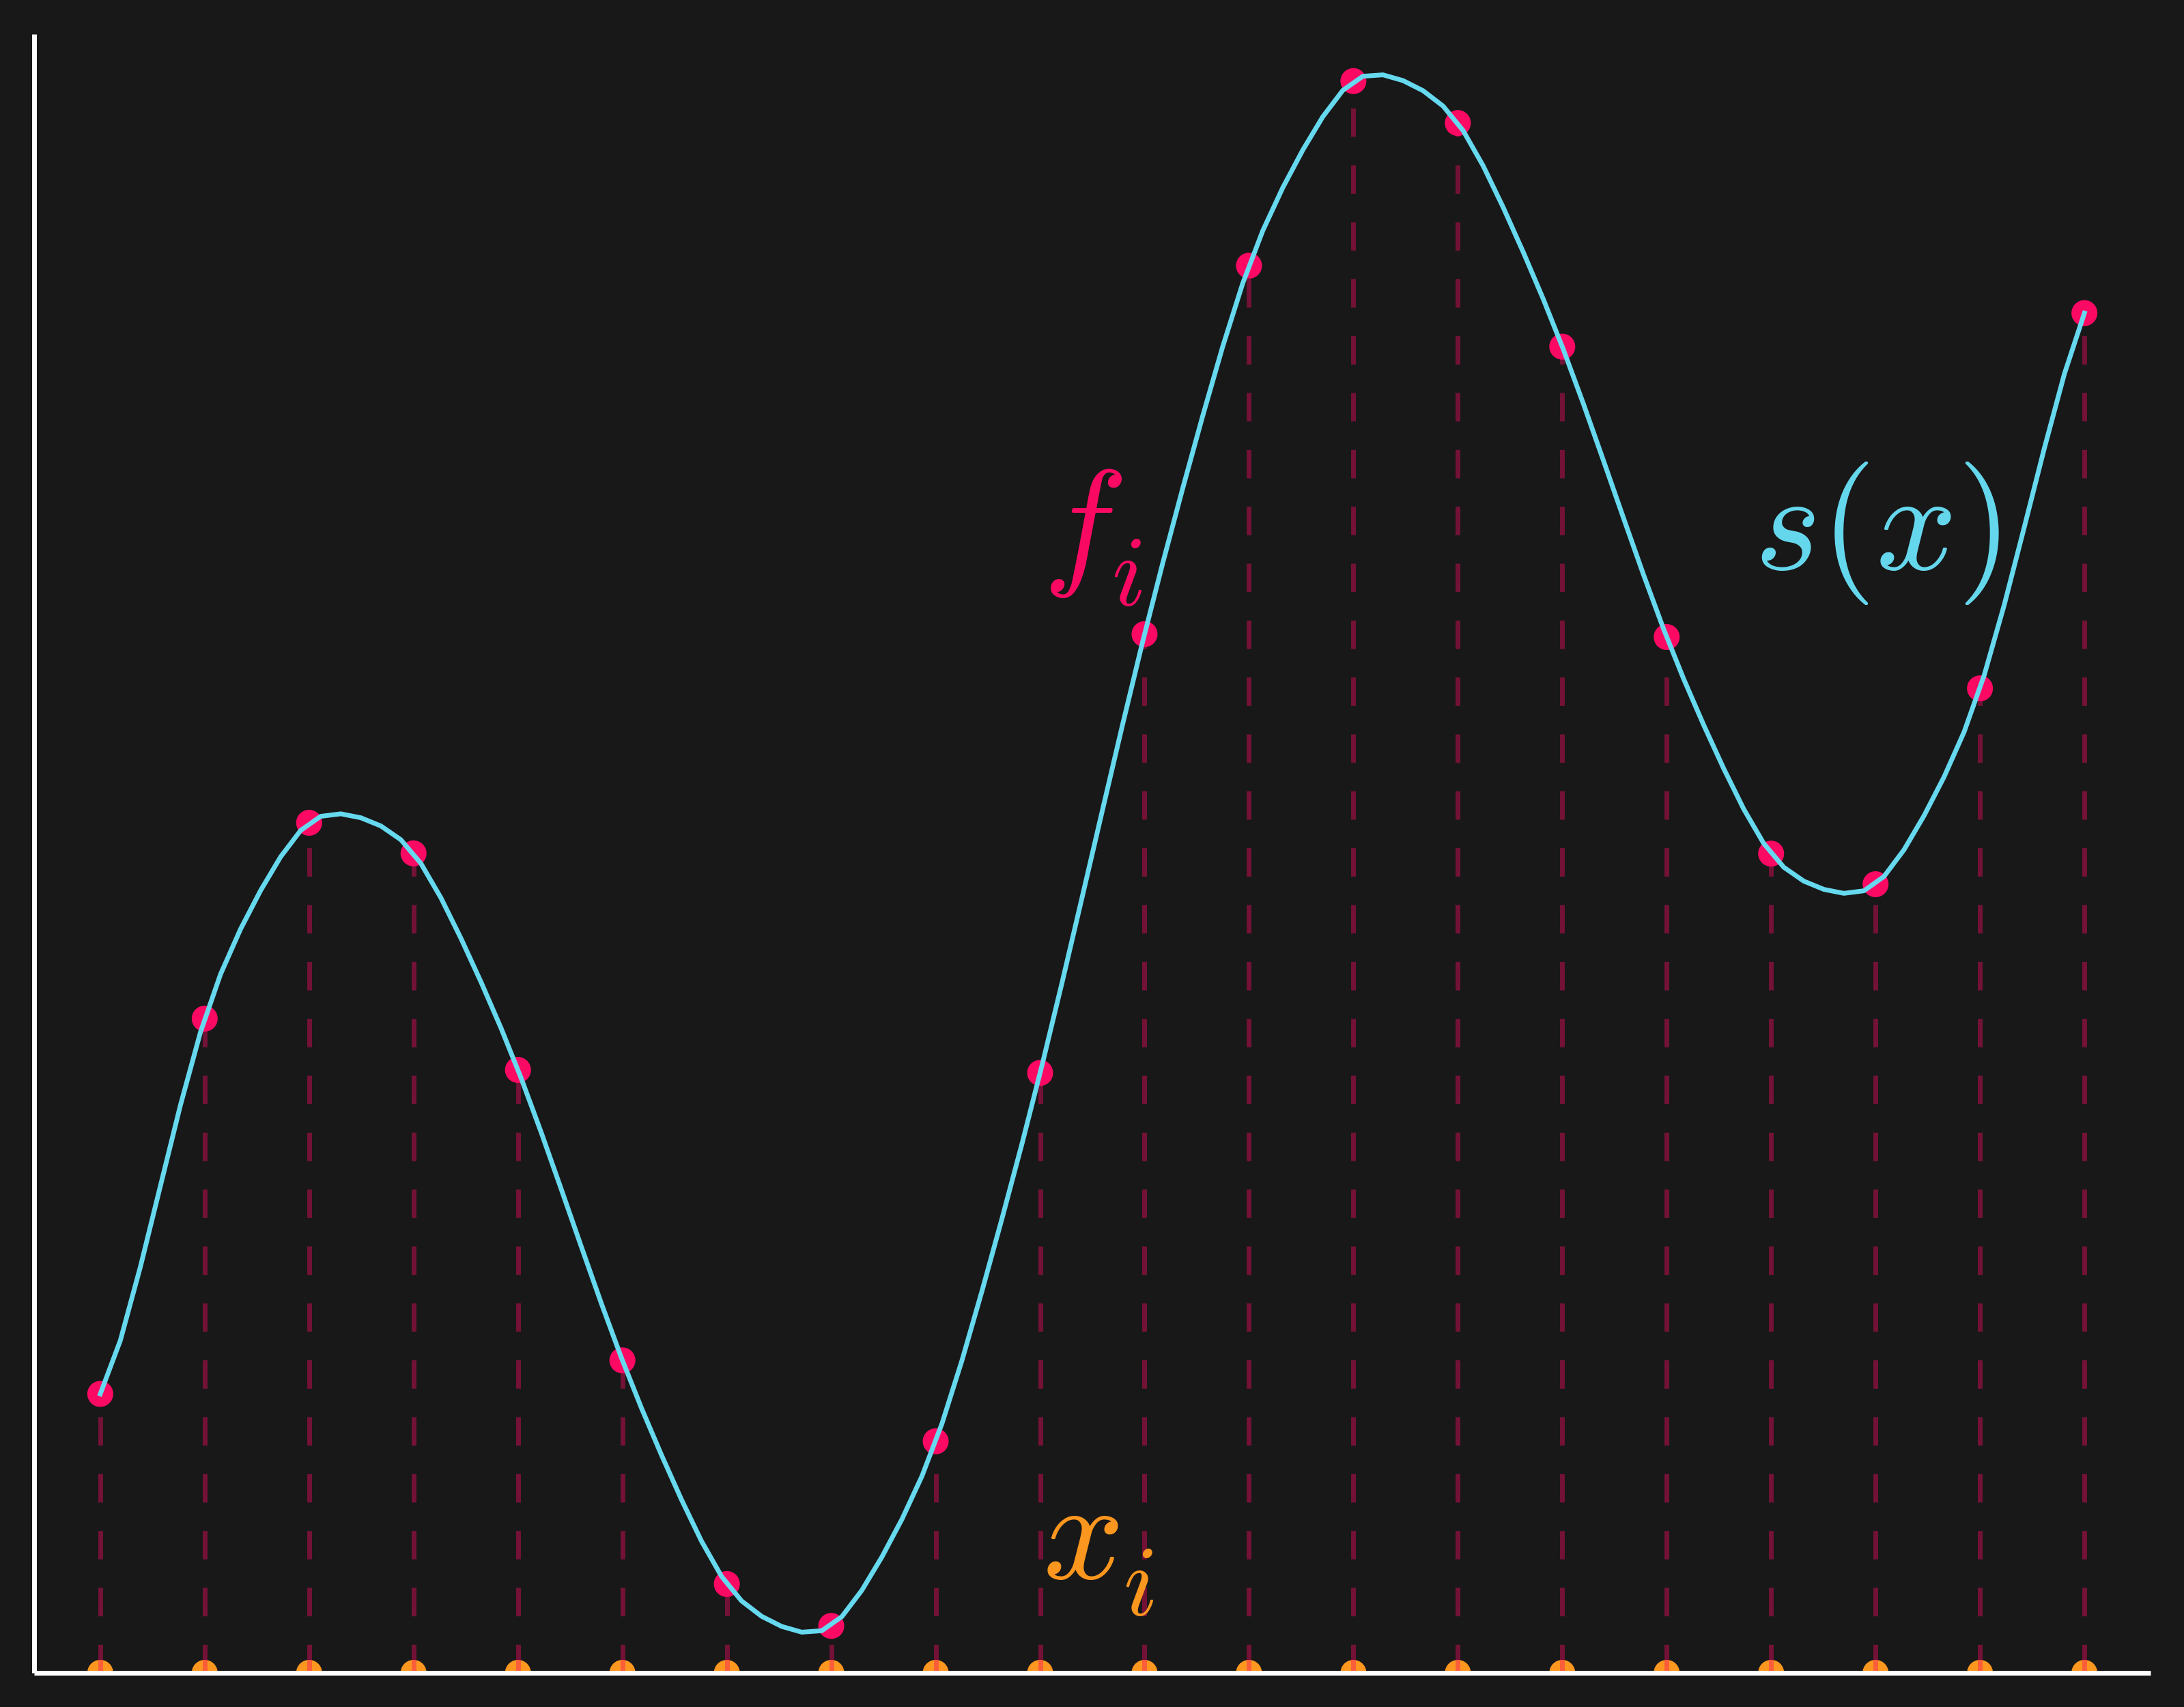
\includegraphics[width=0.7\textwidth, keepaspectratio]{fig1.png}
\end{figure}

\note{}
\end{frame}
\begin{frame}{Motivation}
Given a set of measurments \textcolor{pink}{$\{f_i\}_{i=1}^N$}
taken at corresponding data sites \textcolor{orange}{$\{x_i\}_{i=1}^N$}
we want to find an interpolation function \textcolor{blue}{$s(x)$}
that infroms us on our system at locations different from our data sites.\\
\bigskip 

\subt{Examples of Data Sites and Measurments}
\begin{itemize}
\item[1D:] A series of temperature measurments over a time period
\item[2D:] Surface tempearture of a lake based on measurments collected at sample surface locations 
\item[3D:] Distribution of temperature within a lake
\item[n-D:] Machine learning, financial models, system optimization
\end{itemize}

\note{}
\end{frame}

\begin{frame}{What makes a good fit?}
\bi
\item \textcolor{orange}{Interpolation}: $s(x)$ \subt{exactly matches} our measurments at our data sites. \\ 
\item \textcolor{green}{Approximation}: $s(x)$ \subt{closely matches} our measurments at our data sites, e.g. with Least Squares 
\ei
\begin{figure}
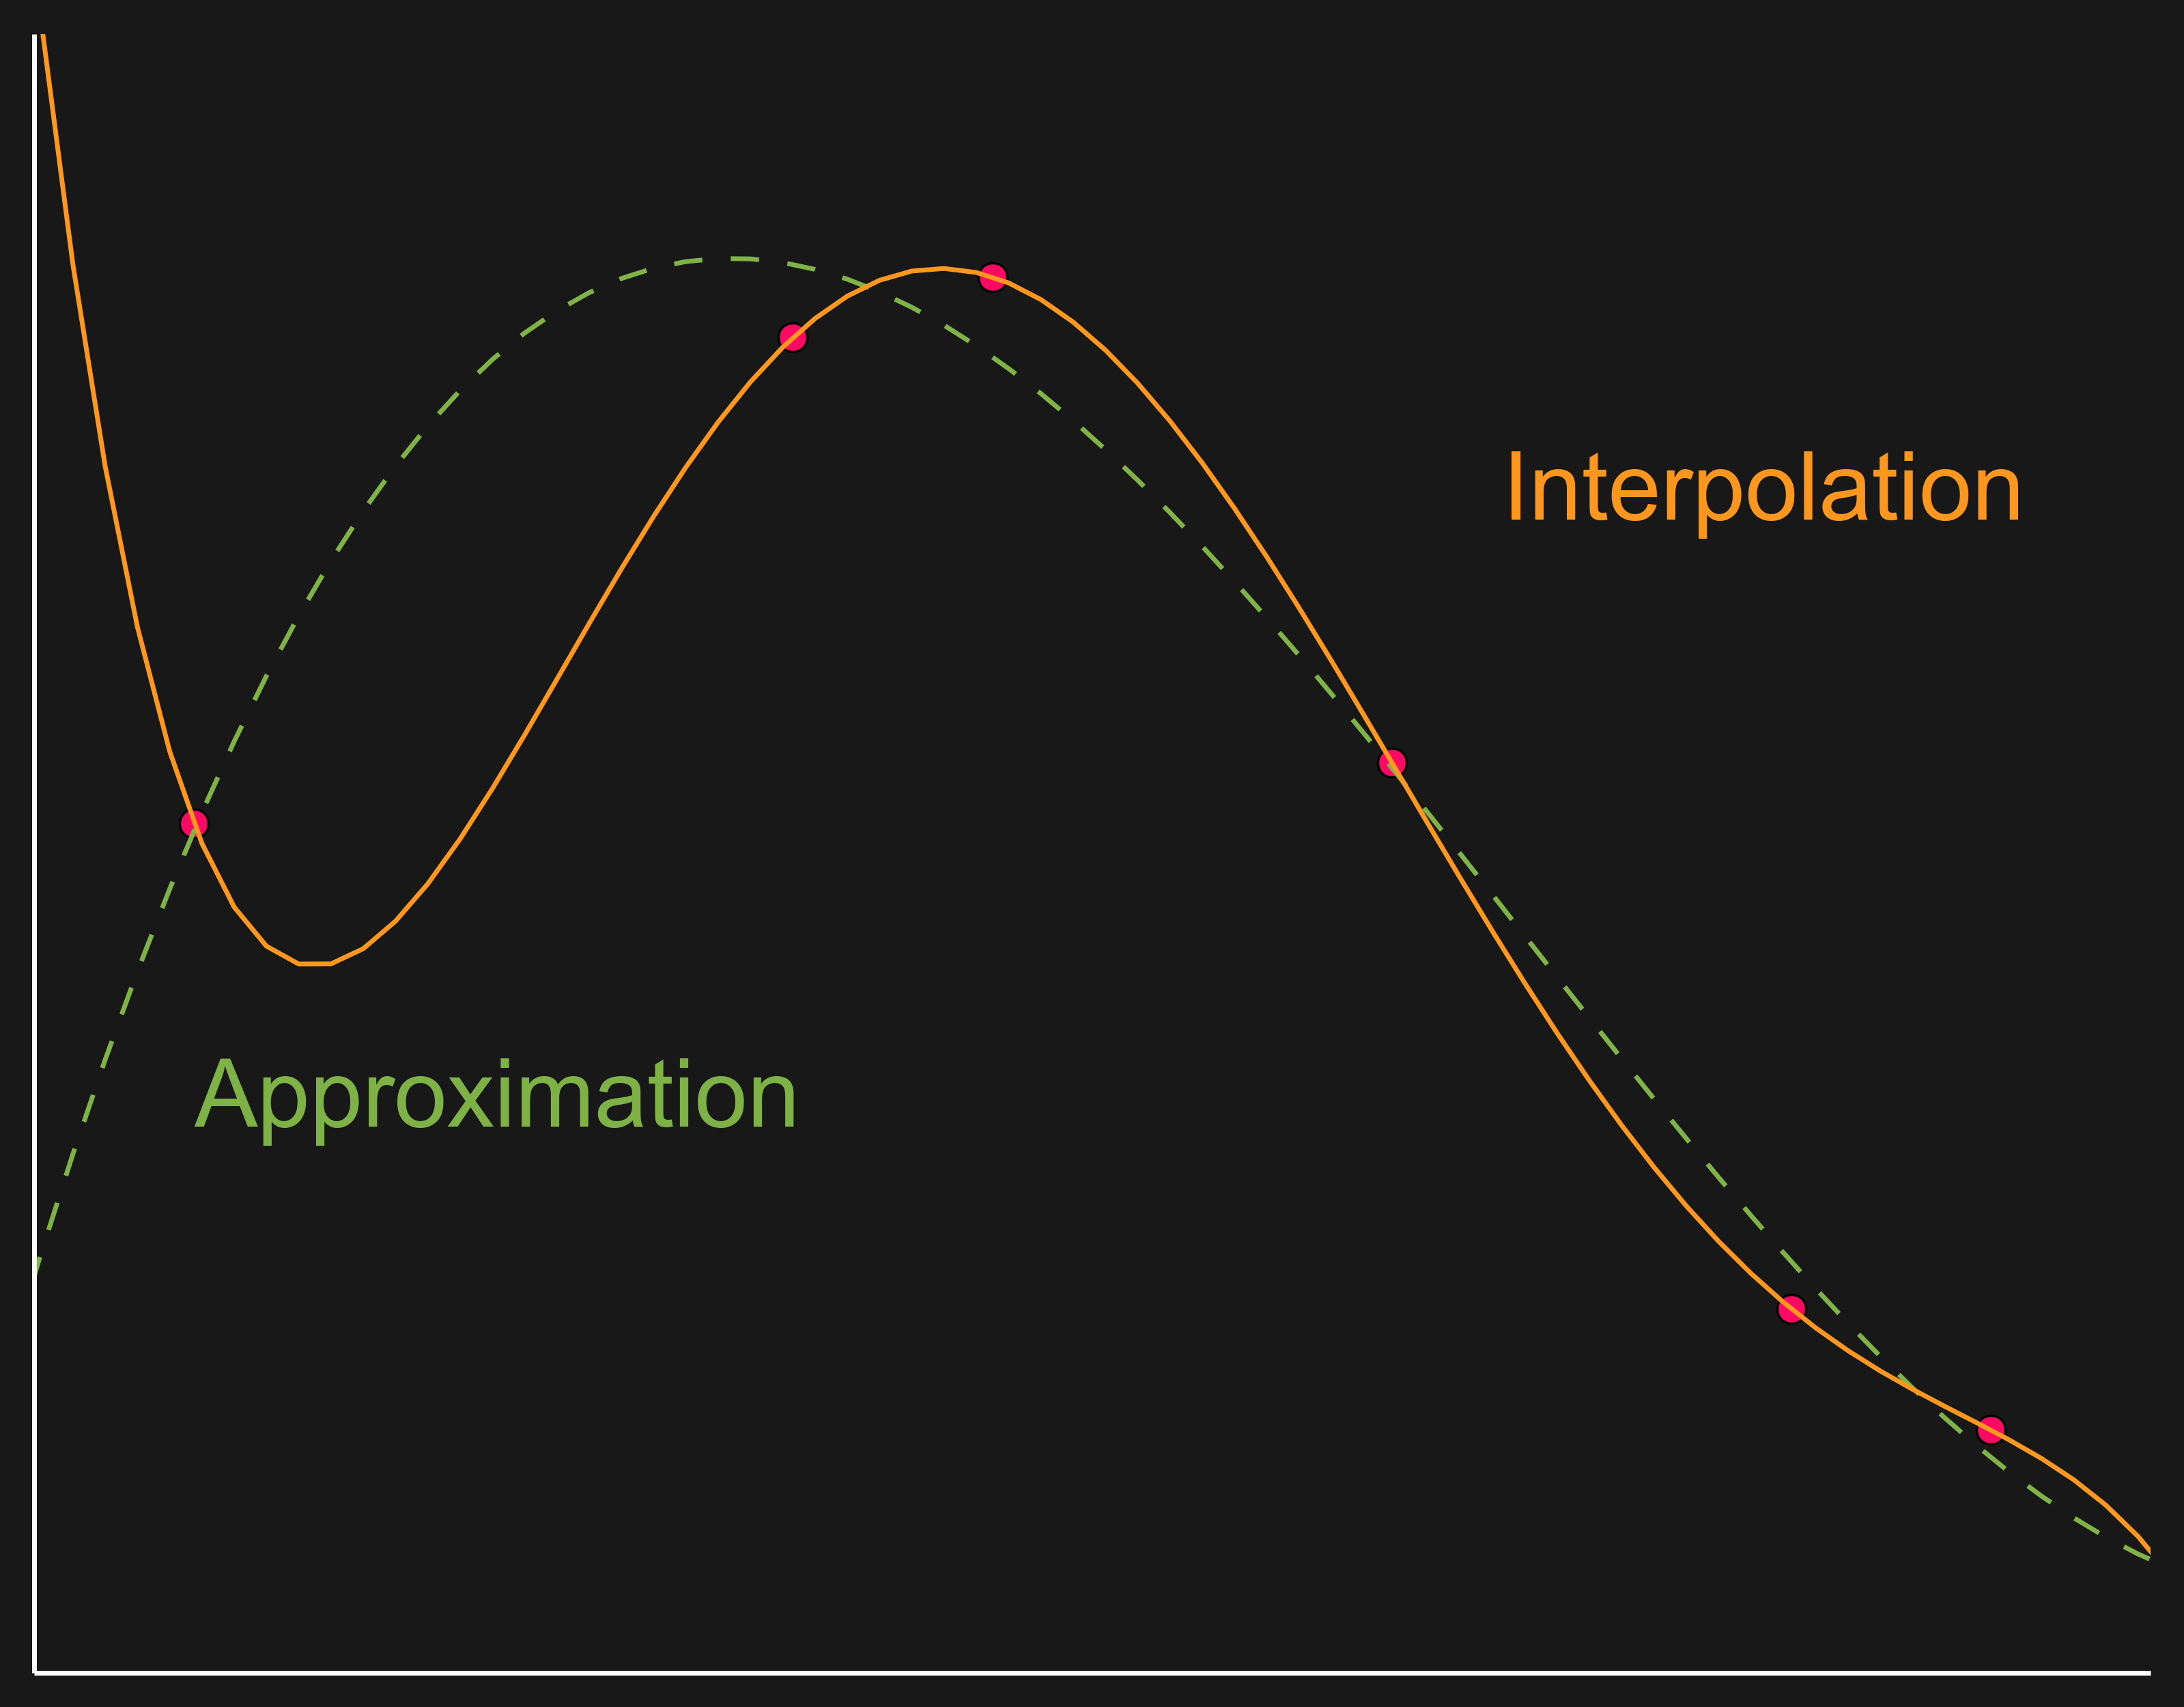
\includegraphics[width=0.7\textwidth, keepaspectratio]{fig2.png}
\end{figure}

\note{}
\end{frame}

\begin{frame}{For today's purposes...}
we will only consider interpolation.

\bi
\item Interpolation: $\textcolor{blue}{s(\textcolor{orange}{x_i})}=\textcolor{pink}{f_i}$ $\forall i\in\{0 \mathellipsis N \}$
\ei
\begin{figure}
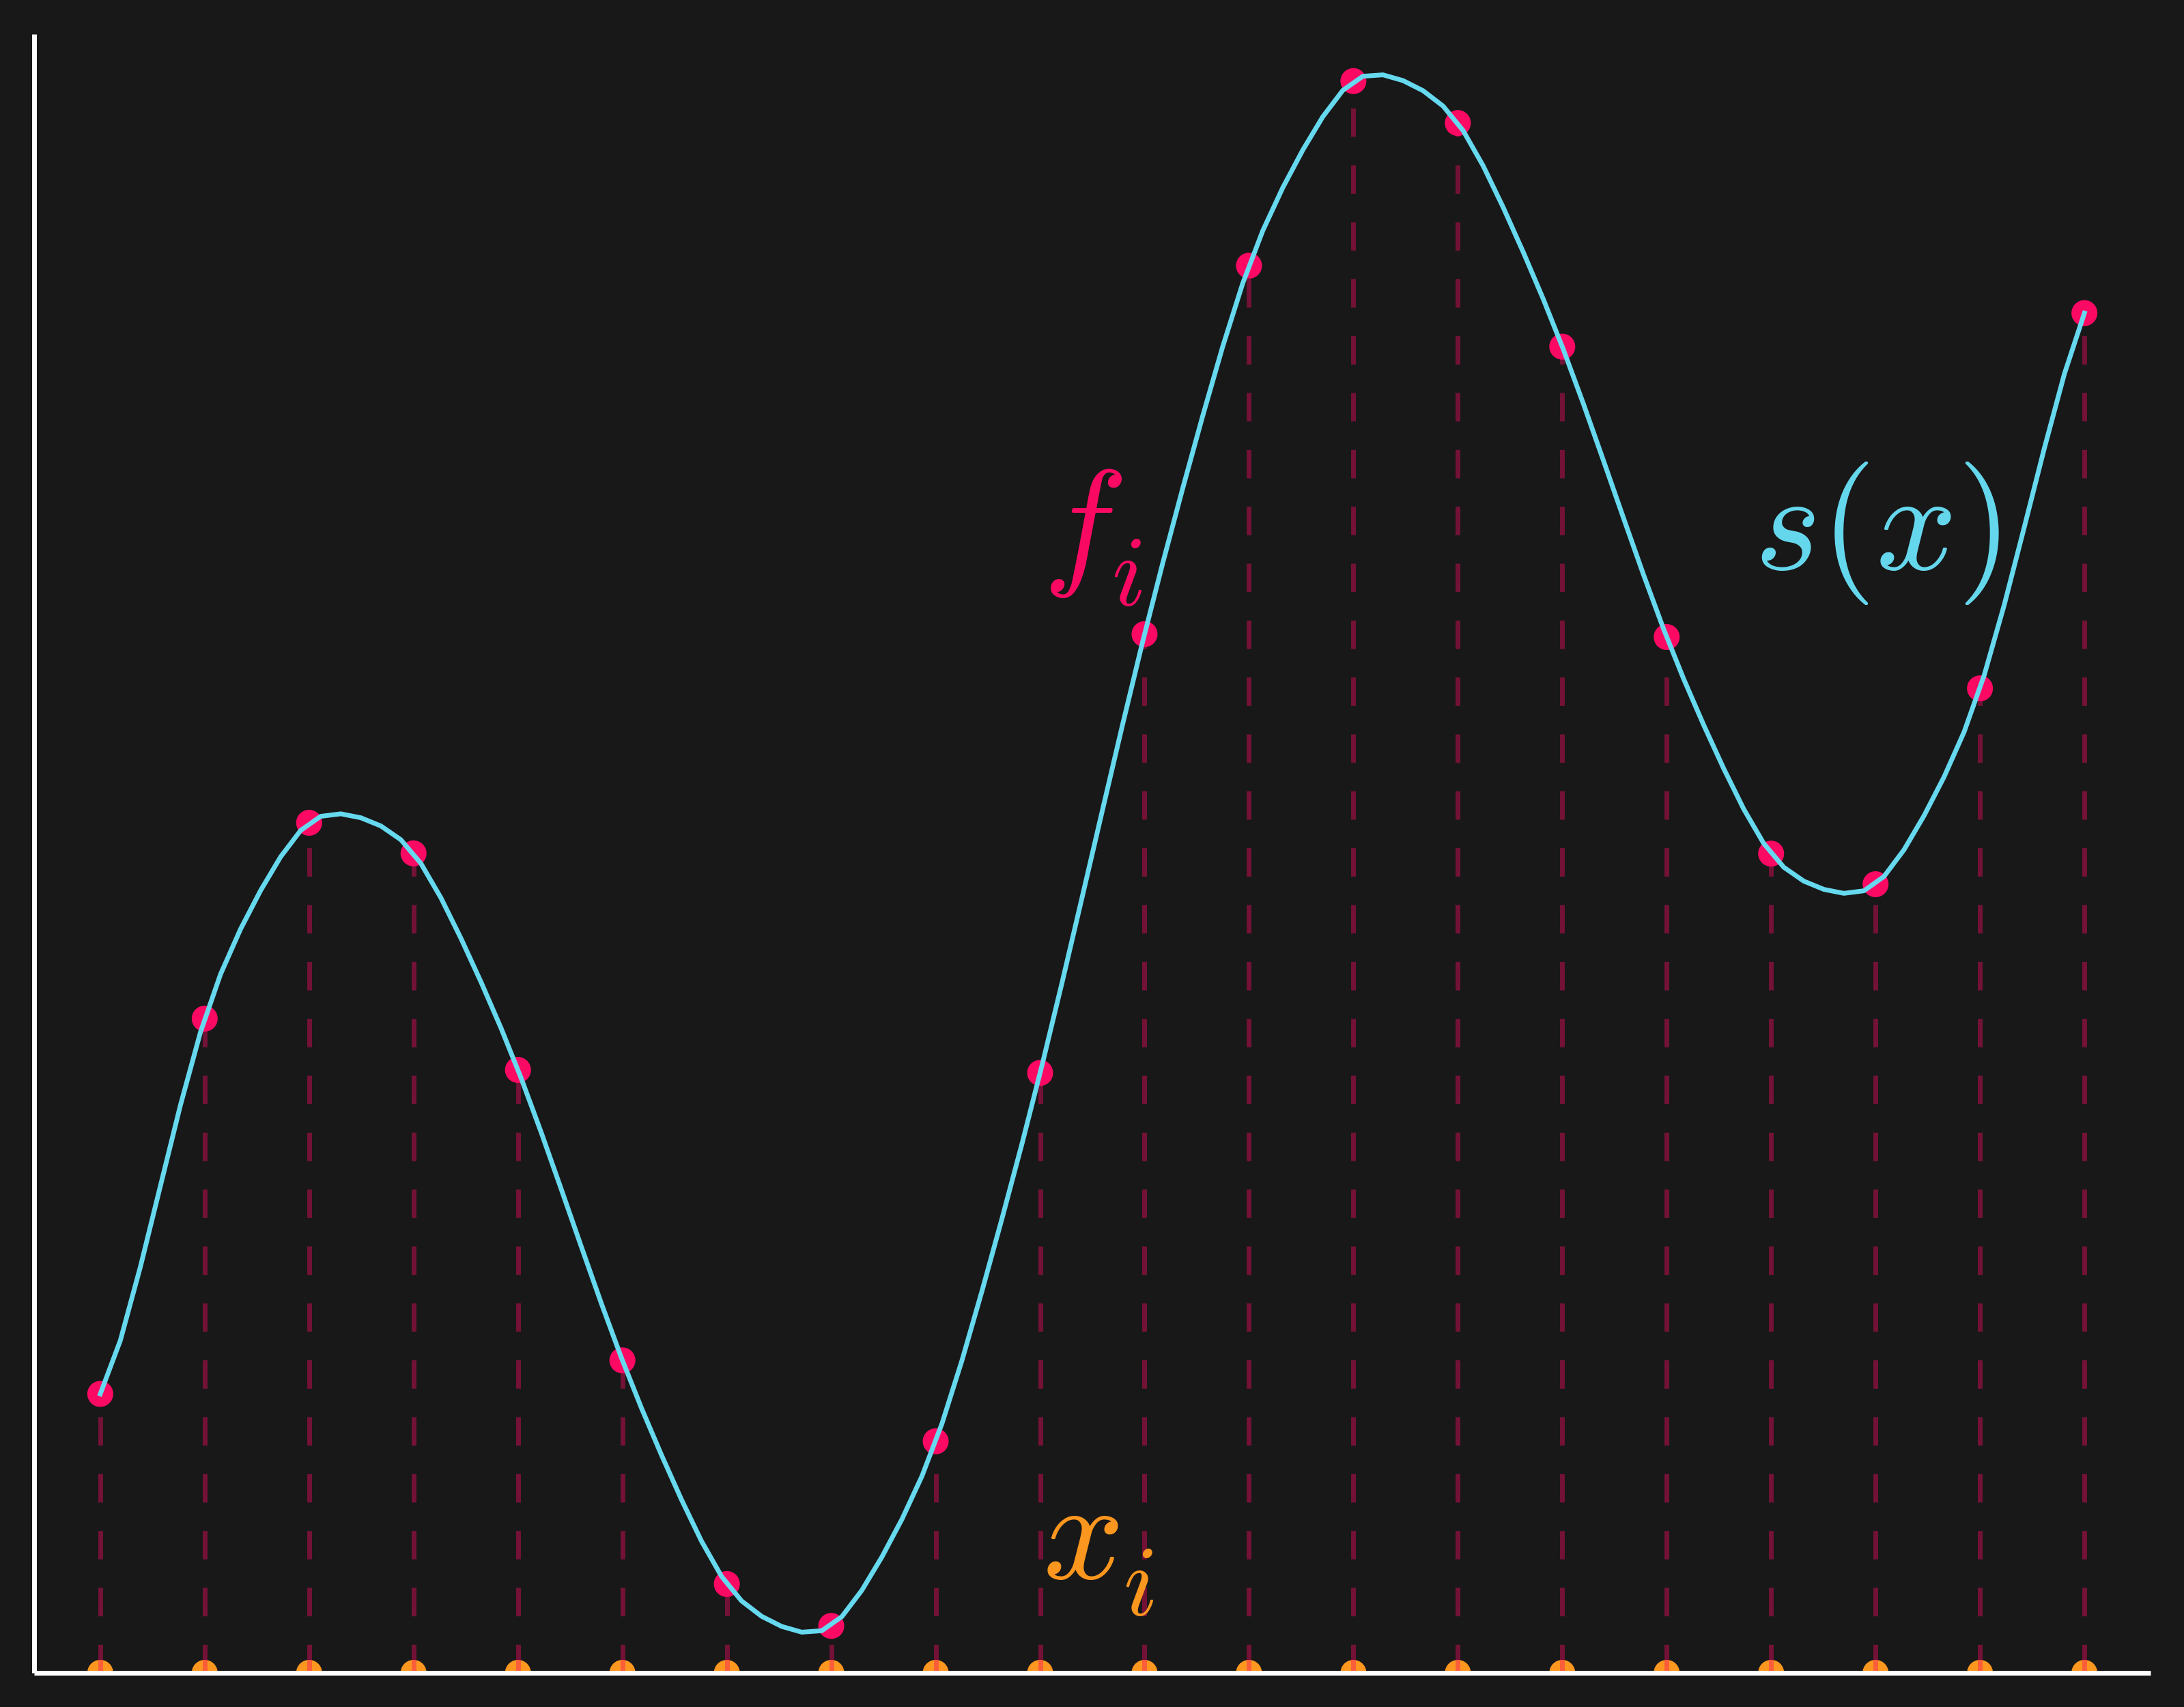
\includegraphics[width=0.7\textwidth, keepaspectratio]{fig1.png}
\end{figure}


\note{}
\end{frame}

\begin{frame}[c]{Our Problem, Restated}

\subt{Interpolation of Scattered Data}

Given data $(\textcolor{orange}{x_i},\textcolor{pink}{f_i})$, $i=1, \mathellipsis, N$, such that $\textcolor{orange}{x_i} \in \mathbb{R}^n$, $\textcolor{pink}{f_i} \in \mathbb{R}$, we want to find a continuous function $\textcolor{blue}{s(x)}$ such that $\textcolor{blue}{s(\textcolor{orange}{x_i})}=\textcolor{pink}{f_i}$ $\forall i\in\{0 \mathellipsis N \}$


\note{}
\end{frame}

\begin{frame}{A Familiar Approach}
\subt{Convenient Assumtption}

Assume $s(x)$ is a linear combination of \subt{basis functions} $\psi_i$
\begin{center}
$s(x)=\sum_{i=1}^N \lambda_i \psi_i$
\end{center}

\subt{Interpolation as a Linear System}

Following this assumption we have a system of linear equations
\begin{center}
$A\boldsymbol{\lambda}=\boldsymbol{f}$
\end{center}
 where
 \bi
\item[A] is called the \subt{interpolation matrix} whose entries are given by\\
\begin{center}
$A_{ii}=\psi_i(x_i)$, $i,i= 1 \mathellipsis N$
\end{center}
\item[$\boldsymbol{\lambda}$] $=\left[ \lambda_1, \mathellipsis, \lambda_N \right]^T$
\item[$\boldsymbol{f}$] $=\left[ f_1, \mathellipsis, f_N \right]^T$
\ei

\note{}
\end{frame}

\begin{frame}{The Well-Posed Problem}
\begin{center}
$A\boldsymbol{\lambda}=\boldsymbol{f}$
\end{center}

Solving this linear system, thus finding $s(x)$, is only possible if the problem \subt{well-posed}, i.e., $\exists$ a unique soltuion. 
\bigskip

\subt{Result from introductory linear algebra:} 

The problem will be well-posed if and only if the interpolation matrix A is \subt{non-singular}, i.e., $\det(A)\neq0$.
\bigskip

\subt{Note:} The non-singularity of A will depend on our choice of basis functions, $\psi_{i=1}^N$

\note{INCLUDE WELL-Conditioned Here!}
\end{frame}

\begin{frame}{Easily Well-Posed in 1D}
In 1D, many choices of basis functions will gauentee a well-posed problem as long as the data-sites are distinct. 
\bigskip

\subt{Example}

We are familiar with \subt{polynomial interpolation}, interpolating from N data sites with a $(N-1)$-degree polynomial. 
\begin{center}
$\psi_{i=1}^N=\{1,x,x^2,x^3, \mathellipsis, x^{N-1}\}$
\end{center}
\begin{figure}
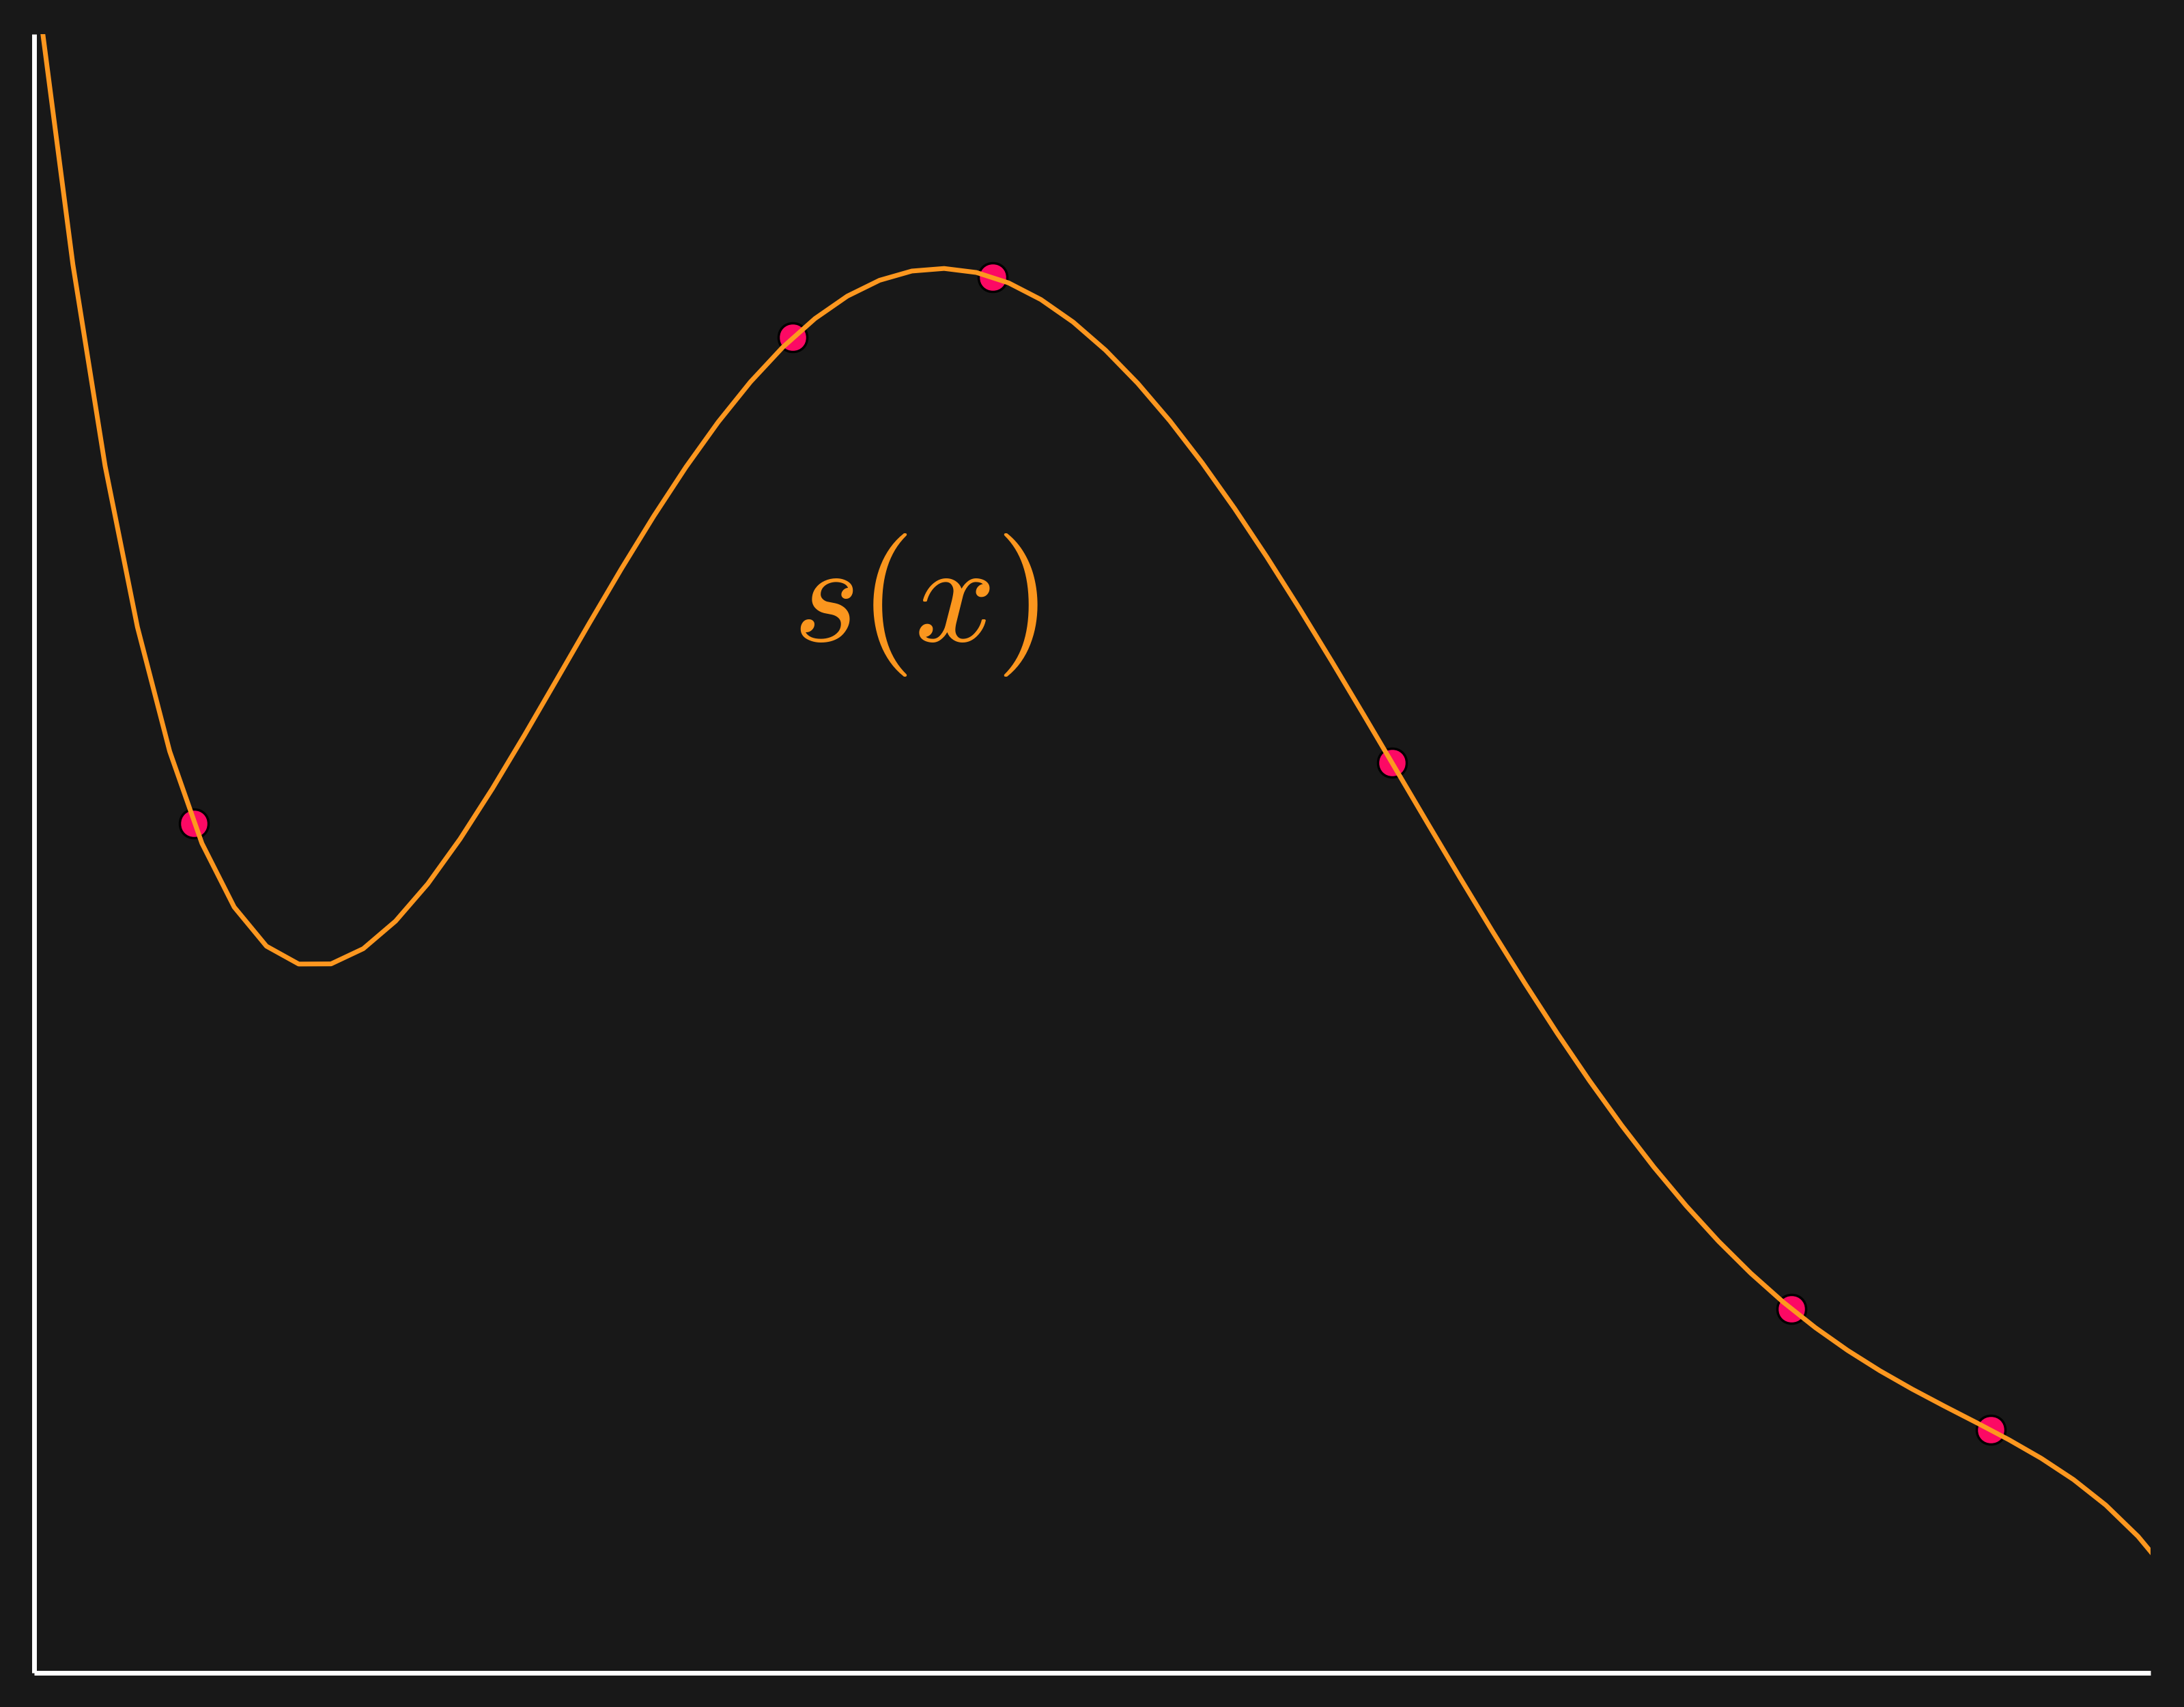
\includegraphics[width=0.4\textwidth, keepaspectratio]{fig3.png}
\end{figure}
\footnotesize{\textcolor{orange}{$s(x)=-0.02988 x^5 + 0.417 x^4 - 2.018 x^3 + 3.694 x^2 - 1.722 x - 5.511e^{-14}$}}
\note{}
\end{frame}

\begin{frame}{A Problem in Higher Dimensions}
For n-Dimensions where $n\geq 2$ there is no such gaurentee.
\bigskip

For any set of basis functions, $\psi_{i=1}^N$ (chosen independently of the data sites) $\exists$ a set of distinct data sites $\{x_i\}_{i=1}^N$
such that the interpolation matrix becomes singular. 
\bigskip

\subt{Implication:}
If we choose our basis functions independently of the data, we are not guarenteed a well-posed problem.
\bigskip

\subt{Note:}
This results from the Haar-Mairhuber-Curtis Theorem


\note{}
\end{frame}

\begin{frame}[c]{A Solution in Higher Dimensions}
\subt{Implication:}
If we choose our basis functions independently of the data, we are not guarenteed a well-posed problem.
\bigskip

\subt{Solution?}

Choose basis functions depending on the data!
\bigskip

\note{}
\end{frame}

\begin{frame}{Basis Functions Depending on Data}
First, consider what we call the \subt{basic function}\\
\begin{equation*}
\psi(x)=|x|
\end{equation*}

\begin{figure}
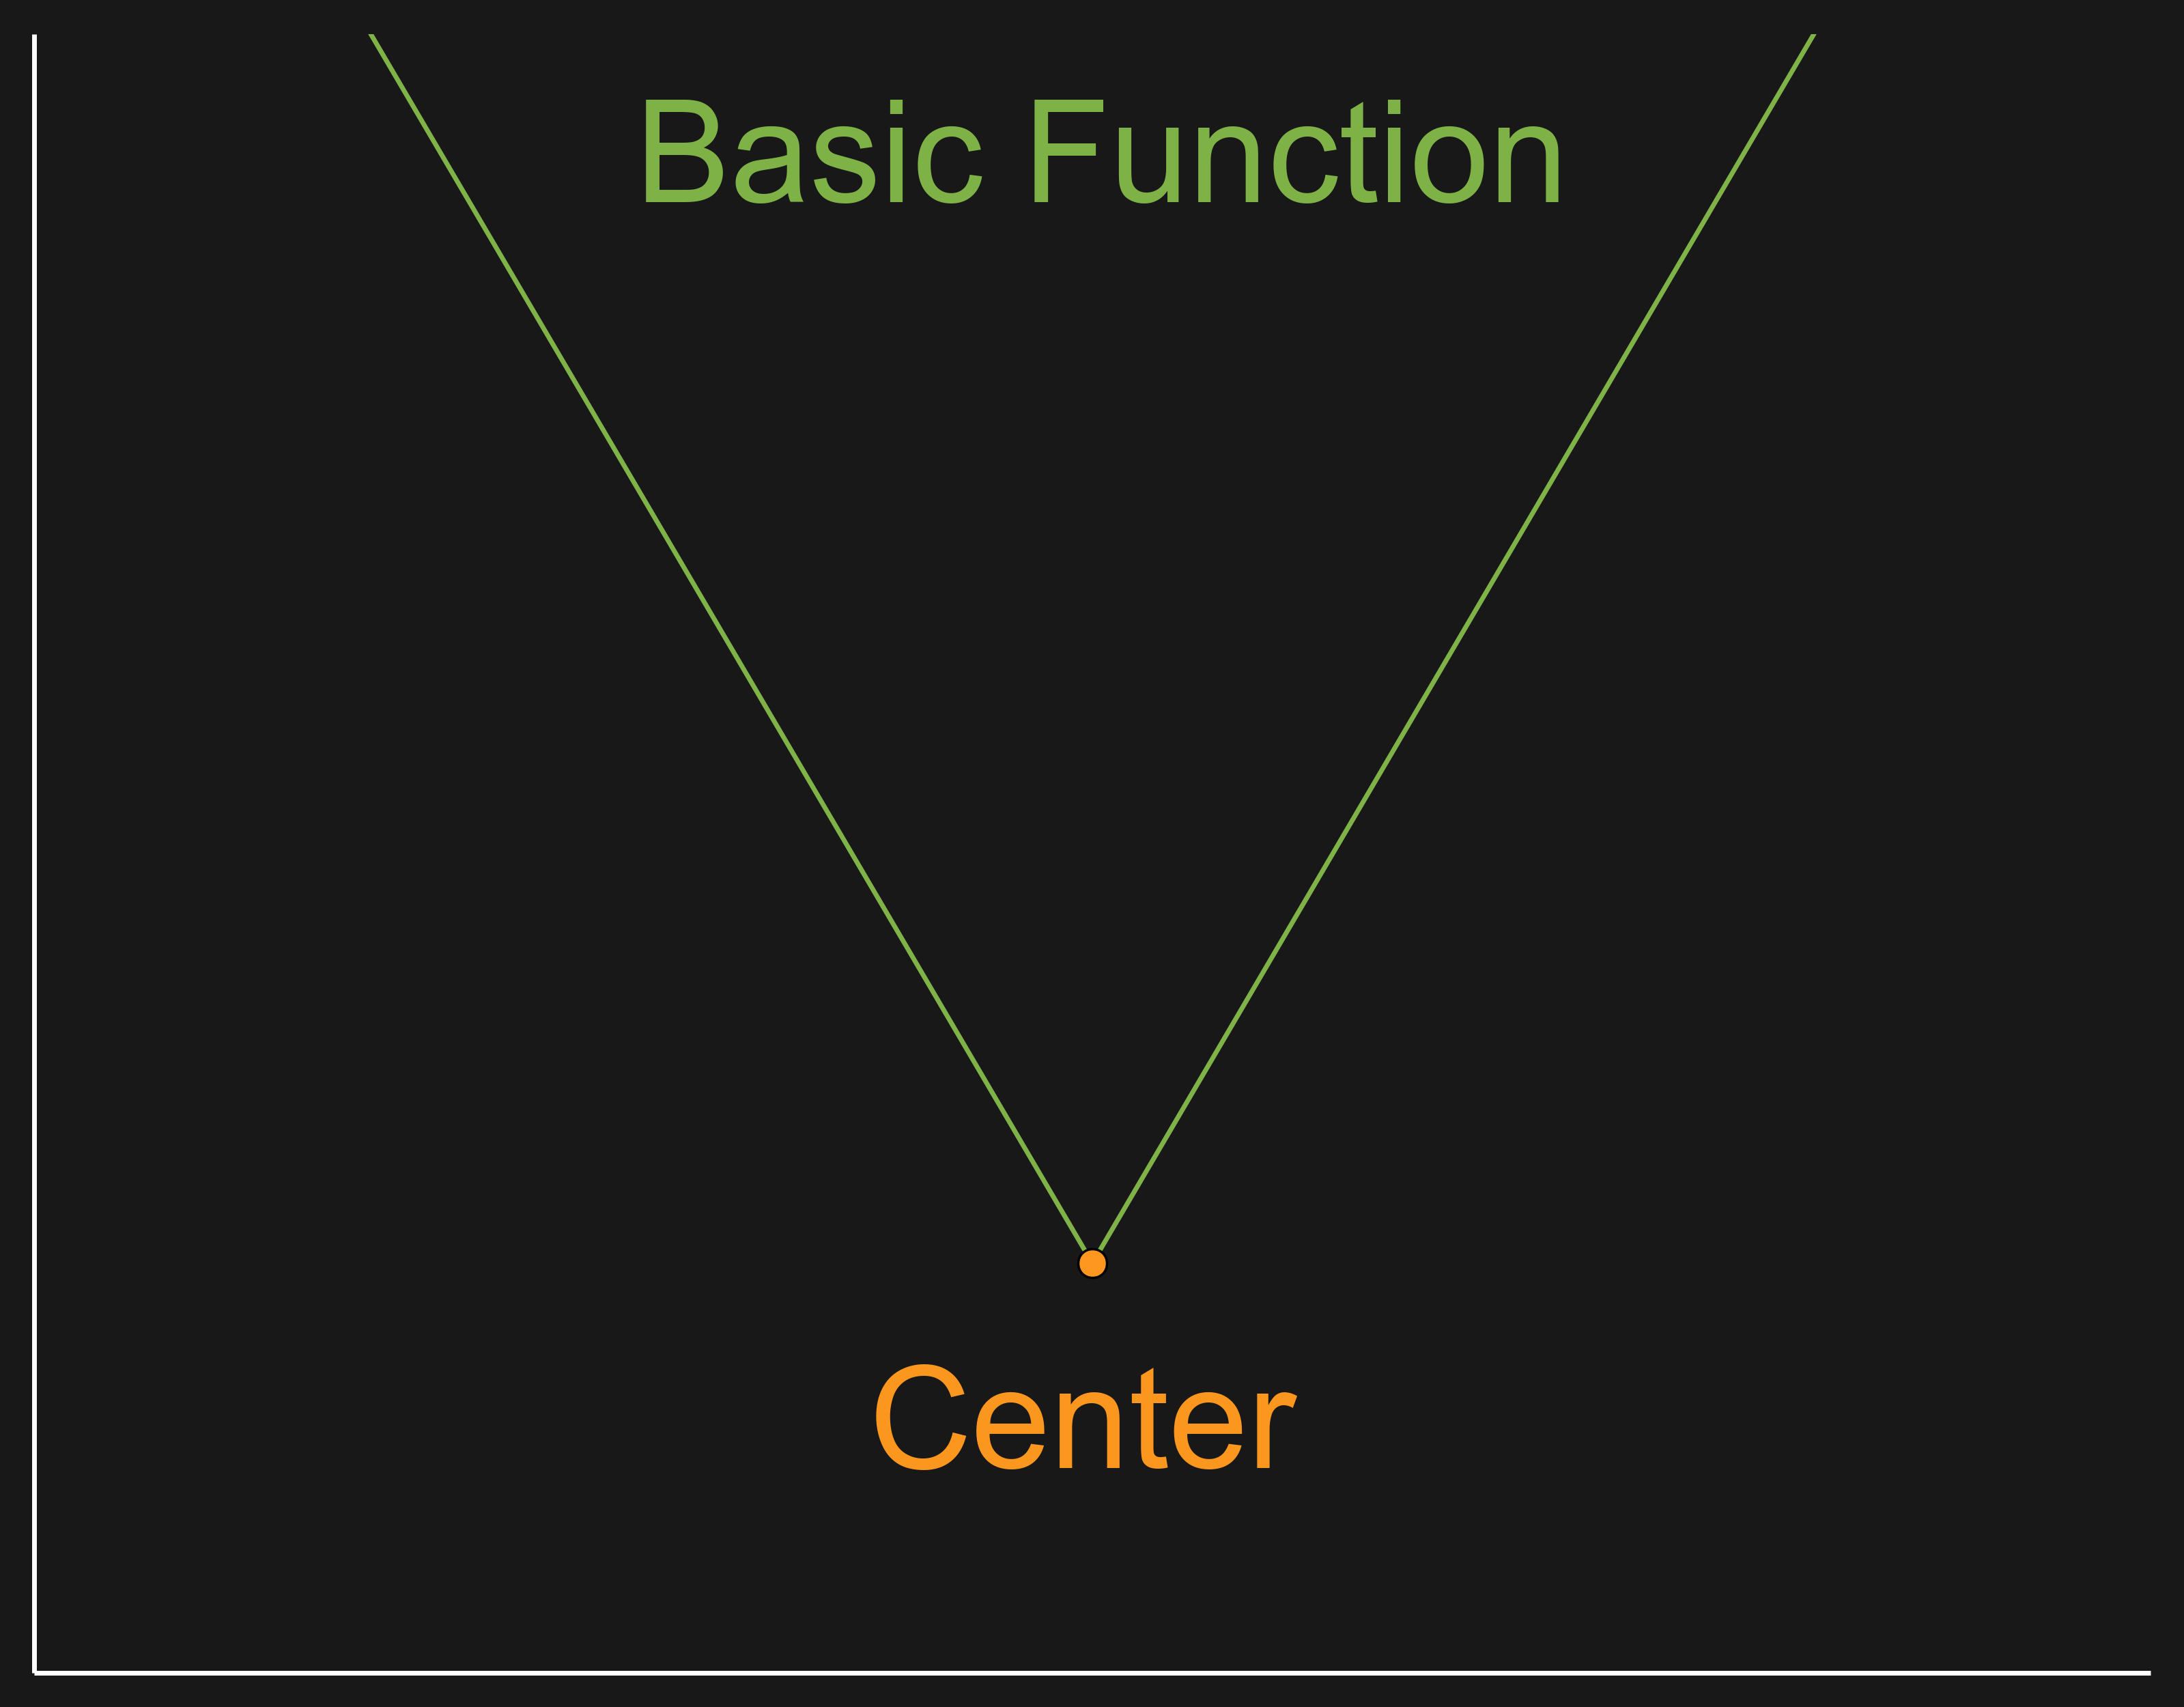
\includegraphics[width=0.7\textwidth, keepaspectratio]{fig4.png}
\end{figure}

\note{Change to || ||
Comment on Radial Symmetry}
\end{frame}

\begin{frame}{Basis Functions Depending on Data}
First, consider what we call the \subt{basic function}\\
\begin{equation*}
\psi(x)=|x|
\end{equation*}

To produce our set of basis functions, we take translates of the basic function.

\begin{equation*}
\psi_i(x)=|x-x_i|, i=1, \mathellipsis, N
\end{equation*}

So each basis function, $\psi_i(x)$, is our basic function shifted so that the \subt{center} or \subt{knot} is positioned on a data site, $x_i$.
\bigskip

\subt{Note:} It's possible to have other choices of centers, but in most implementations the centers coincide with data sites.

\note{Change to || ||
Comment on Radial Symmetry}
\end{frame}

\begin{frame}{Basis Functions Depending on Data}

To produce our set of basis functions, we take translates of the basic function.

\begin{equation*}
\psi_i(x)=|x-x_i|, i=1, \mathellipsis, N
\end{equation*}

So each basis function, $\psi_i(x)$, is our basic function shifted so that the \subt{center} or \subt{knot} is positioned on a data site, $x_i$.




\note{Change to || ||
Comment on Radial Symmetry}
\end{frame}

\begin{frame}{Radial Basis Functions}

\begin{equation*}
\psi_i(x)=|x-x_i|, i=1, \mathellipsis, N
\end{equation*}

Notice that $\psi_k(x)$ are radially symmetric about their centers, for this reason we call these functions \subt{Radial Basis Functions}.
\bigskip

Since the basis functions only depend on distance, the interpolation matrix becomes
\begin{equation*}
A=
\begin{bmatrix}
|x_1-x_1| & |x_1-x_2| & \cdots & |x_1-x_N|\\
|x_2-x_1| & |x_2-x_2|& \cdots & |x_2-x_N|\\
\vdots & \vdots & \ddots & \vdots\\
|x_N-x_1| & |x_N-x_2|& \cdots & |x_N-x_N|
\end{bmatrix}
\end{equation*}
called a \subt{distance matrix}.

\note{}
\end{frame}

\begin{frame}{The Distance Matrix}
Distance matricies have the property that, for Euclidean distances in any dimensions, the distance matrix is non-singular.
\bigskip

This means that our interpolation problem

\begin{equation*}
\begin{bmatrix}
||x_1-x_1|| & ||x_1-x_2|| & \cdots & ||x_1-x_N||\\
||x_2-x_1|| & ||x_2-x_2||& \cdots & ||x_2-x_N||\\
\vdots & \vdots & \ddots & \vdots\\
||x_N-x_1|| & ||x_N-x_2||& \cdots & ||x_N-x_N||
\end{bmatrix}
\begin{bmatrix}
\lambda_1\\
\lambda_2\\
\vdots\\
\lambda_N
\end{bmatrix}
=
\begin{bmatrix}
f_1\\
f_2\\
\vdots\\
f_N
\end{bmatrix}
\end{equation*}
is well-posed!
\bigskip

Our interpolant becomes 
\subt{$s(x)=\sum_{i=1}^N \lambda_i ||x-x_i|| $}

\note{}
\end{frame}

\begin{frame}{Building a Better Basic Function}
However, $\psi_i(x)=||x-x_i||$ has a discontinuity in its first derivative at $x_i$. This causes the interpolant to have a discontinuous first derivative at each data site. This is obviously not ideal.
\bigskip

In 1968, R.L. Hardy showed that we can remedy this problem by changing our basic function to one with continuous derivatives.

\subt{Hardy's Multiquadrc Kernel}
\begin{equation*}
\psi(x)=\sqrt{\epsilon^2 + x^2}
\end{equation*}
where $\epsilon > 0$.

\subt{Note:} The case where $\epsilon=0$ is just the previous basic function.

\note{}
\end{frame}

\begin{frame}{Radial Basis Kernels}
As before, we can generate our basis functions by translating Hardy's basic function to center on our data sites.
\begin{equation*}
\psi_i(x)=\sqrt{\epsilon^2 + (||x-x_i||)^2}
\end{equation*}

Notice that the Hardy's Multiquadric function is still radially symetric about its center, making it a Radial Basis Function (RBF). 
All RBFs are functions only of distance from center, and can be written generally as $\phi(||x-x_i||)$

\subt{The RBF Method}
\begin{equation*}
s(x)=\sum_{i=1}^N \lambda_i \phi(||x-x_i||)
\end{equation*}

\note{}
\end{frame}

\begin{frame}{Radial Basis Kernels}

\subt{The RBF Method}
\begin{equation*}
s(x)=\sum_{i=1}^N \lambda_i \phi(||x-x_i||)
\end{equation*}

There are a few commonly used RBF Kernels:

% \begin{tabular}
% test & test\\
% test & test
% \end{tabular}

\note{Graphs of each kernel!}
\end{frame}

\end{document}